\chapter{Condizionamento dell'Ingresso}

%--------------------------------------------------------------------------------------------

\section{Convertitore Lineare-Esponenziale}

%--------------------------------------------------------------------------------------------

Vogliamo ora analizzare la sezione di circuto che soddisfa la specifica sulla modalità
$1V/Octave$ dell'ingresso, ovvero il circuito in grado di convertire una tensione
lineare in una esponenziale.

Il circuito utilizzato è molto diffuso in questo tipo di applicazioni, si può infatti
trovare in molti siti di DIY come quello di René Schmitz \cite{expo_converter}, personaggio
molto noto tra gli appassionati di sintetizzatori musicali fai-da-te.

%--------------------------------------------------------------------------------------------

\subsection*{Analisi del Circuito}

%--------------------------------------------------------------------------------------------

Per l'applicazione si sfrutta la caratteristica esponenziale intrinseca del transistor
bipolare:

\begin{displaymath}
    I_e\approx I_c=I_se^{\left(\frac{V_{be}}{V_T}-1\right)}
    \approx I_se^{\left(\frac{V_{be}}{V_T}\right)}
\end{displaymath}

\begin{figure}[ht]
    \centering
    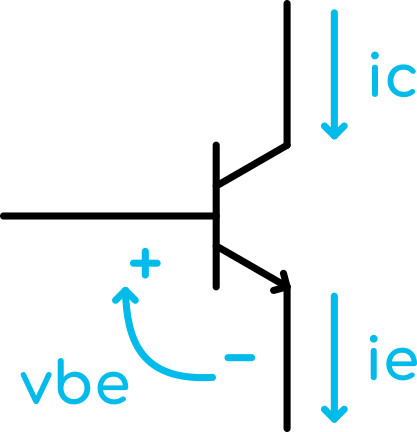
\includegraphics{circuits/single_transistor_circuit.png}
    \caption{BJT}
    \label{bjt}
\end{figure}

dove $V_T$ (o potenziale termico) e $I_s$ (o corrente di saturazione) sono variabili in
funzione della temperatura, anche se nella nostra analisi $V_T$ verrà considerato di
valore costante pari a $26mV$.

Per rimuovere dall'equazione $I_s$, che invece risulta molto più problematico, si collega
una coppia di transistor (idealmente nello stesso chip, in modo che siano il più possibile
simili tra loro e termicamente accoppiati) in configurazione differenziale:
\medskip

\begin{figure}[ht]
    \centering
    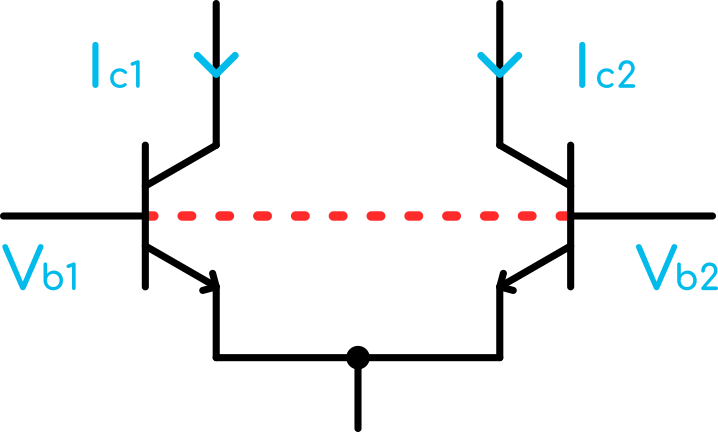
\includegraphics{circuits/differential_pair_circuit.png}
    \caption{Coppia differenziale a BJT}
    \label{differential_pair_circuit}
\end{figure}

per la quale possiamo scrivere la seguente relazione:

\begin{displaymath}
    \frac{I_{c2}}{I_{c1}}=\frac{I_s e^{\left(\frac{V_{be2}}{V_T}\right)}}{I_s e^{\left(\frac{V_{be1}}{V_T}\right)}}
    \qquad
    \rightarrow
    \qquad
    I_{c2}=I_{c1}e^{\left(\frac{V_{be2}-V_{be1}}{V_T}\right)}=I_{c1}e^{\left(\frac{V_{b2}-V_{b1}}{V_T}\right)}
\end{displaymath}

in cui risulta evidente che la dipendenza da $I_s$ viene completamente rimossa.

A questo punto, apportiamo alcune modifiche al circuito, ottenendo dunque il seguente:
\medskip

\begin{figure}[ht]
    \centering
    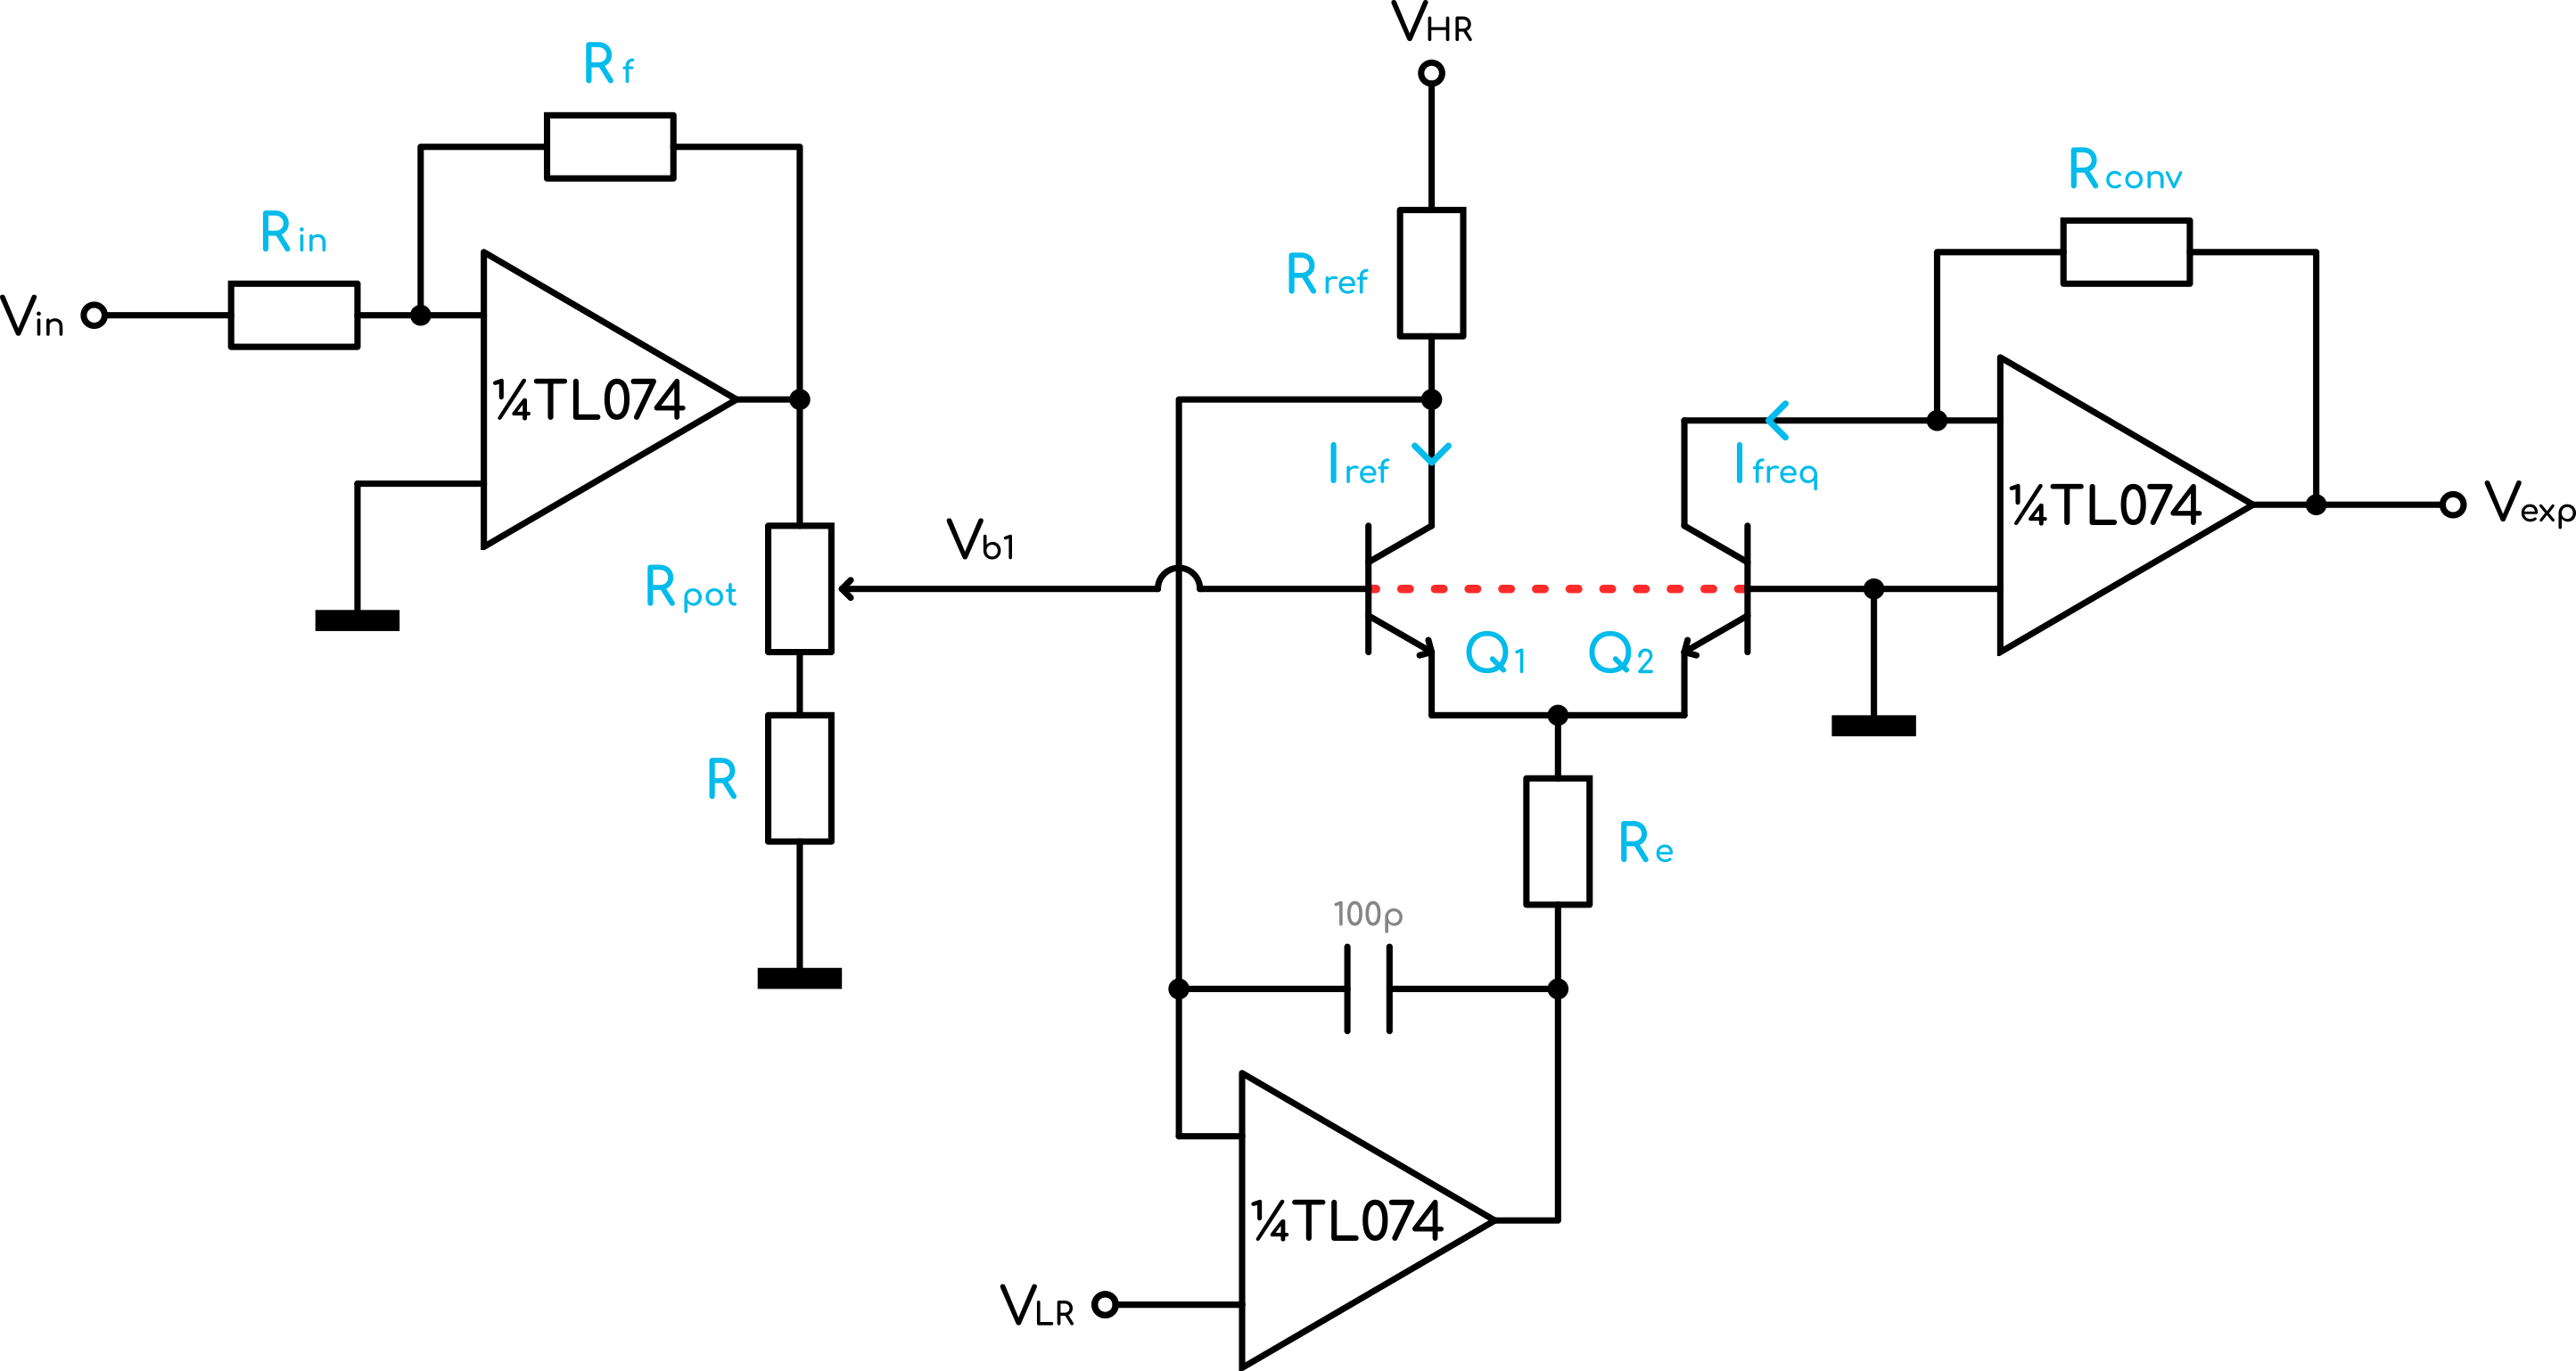
\includegraphics{circuits/exponential_converter_circuit.png}
    \caption{Schema elettrico di un convertitore tensione lineare - corrente esponenziale}
    \label{exponential_converter_circuit}
\end{figure}

che ci permette di legare ingresso e uscita tramite le relazioni

\begin{displaymath}
    i_{freq}=I_{ref}e^{\left(-\frac{v_{b1}}{V_T}\right)}
\end{displaymath}

\begin{displaymath}
    I_{ref}=\frac{V_{HR}-V_{LR}}{R_{ref}}
\end{displaymath}

L'operazionale di sinistra (rappresentato in figura \ref{exponential_converter_circuit})
si occupa di invertire il segno della tensione di ingresso e portarla in un rage appropriato
per la base del transistor, questo consente di avere un valore positivo all'esponente. Quello
di destra invece, si occupa di mantenere costante la corrente di riferimento $I_{ref}$.

Si aggiunge ora un semplice convertitore corrente-tensione al collettore di $Q_2$, quindi:

\begin{displaymath}
    V_{out}=R_f\cdot i_{freq}=
    R_f\cdot \frac{V_{HR}-V_{LR}}{R_{ref}}e^{\left(-\frac{s\cdot V_{in}}{V_T}\right)}
\end{displaymath}

% circuito completo con IVC figura 4

%--------------------------------------------------------------------------------------------

\subsection*{Dimensionamento e Scelta dei Componenti}

%--------------------------------------------------------------------------------------------

Passiamo quindi al dimensionamento dei componenti, in modo da imporre al circuito il
comportamento voluto.

Come prima cosa calcoliamo il valore del guadagno $s$ dell'amplificatore invertente.
Si vuole:

\begin{displaymath}
    i_{freq}=I_{ref}e^{-\frac{s\cdot V_{in}}{V_T}}
    \qquad
    \rightarrow
    \qquad
    2i_{freq}=I_{ref}e^{-\frac{s\cdot[V_{in}+\Delta V_{in}]}{V_T}}
\end{displaymath}

qundi un raddoppio della corrente $i_{freq}$ per ogni variazione $\Delta V_{in}=1V$.
Allora possiamo riscrivere le due relazioni nel seguente modo:

\begin{displaymath}
    2=e^{-\frac{s\cdot\Delta V_{in}}{V_T}}
    \qquad
    \rightarrow
    \qquad
    ln(2)=-\frac{s\cdot\Delta V_{in}}{V_T}
    \qquad
    \rightarrow
    \qquad
    -s=\frac{V_T\cdot ln(2)}{\Delta V_{in}}
\end{displaymath}

e sostituendo i valori otteniamo:

\begin{displaymath}
    -s=\frac{26mV\cdot 0.6931}{1V}\approx-0.018\approx-\frac{1}{55.5}
\end{displaymath}

valore che può essere diviso nel seguente modo:

\begin{displaymath}
    s=\bar{s}\cdot\hat{s}=\frac{2k\Omega}{100k\Omega}\cdot\frac{440\Omega}{490\Omega}
    \approx 0.018
\end{displaymath}

quindi:

% circuito amplificatore completo figura 5

\begin{itemize}
    \item $R_f = 2k\Omega$;
    \item $R_{in} = 100k\Omega$;
    \item $R_{pot} = 100\Omega$;
    \item $R = 390\Omega$;
\end{itemize}

impostiamo i valori di $V_{HR}=+12V$ e $V_{LR}=0V$.

%--------------------------------------------------------------------------------------------

\subsection*{Risultati Pratici e Misure}

%--------------------------------------------------------------------------------------------

testo

%--------------------------------------------------------------------------------------------

\section{Somma di più Ingressi}

%--------------------------------------------------------------------------------------------

testo

%--------------------------------------------------------------------------------------------

\section{Clipper}

%--------------------------------------------------------------------------------------------

testo

%--------------------------------------------------------------------------------------------

\subsection*{Risultati Pratici e Misure}

%--------------------------------------------------------------------------------------------
